Un haz luminoso estrecho de luz, $AO$, incide en un espejo plano $E_1$, de manera que el haz reflejado, $OB$, sea perpendicular a $AO$, como se ilustra en la figura de esta pregunta. Otro espejo plano $E_2$ debe colocarse dentro del rectángulo indicado con líneas no continuas, de manera que el haz $OB$ se refleje en la dirección $CD$, paralela a $AO$. El espejo $E_2$, debe, entonces, colocarse:\\
\textit{a}) Paralelamente a $AO$. \textit{b}) Perpendicularmente a $AO$. \textit{c}) Perpendicularmente a $E_1$. \textit{d}) Paralelamente a $E_1$. \textit{e}) Formando un ángulo de 45$^o$ con $E_1$.
\begin{figure}[h!]
  \centering
  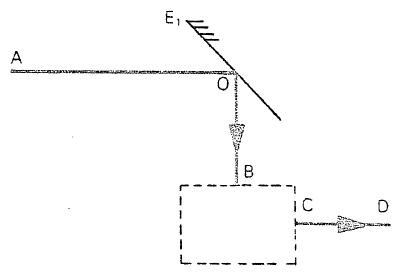
\includegraphics[scale=0.47]{figuras/fig_alvarenga_p653_9.png}
  \caption{Problema 17}
\end{figure}